\documentclass[aps,pre,twocolumn,showpacs,superscriptaddress,groupedaddress]{revtex4-1}

\usepackage{graphicx}
\usepackage{amsmath}
\usepackage{amssymb}
\usepackage{color}
\usepackage{bm}
\usepackage{hyperref}
\usepackage{epsfig}
\usepackage{subfigure}

\begin{document}

\title{Synchronization Transitions in Coupled Kardar-Parisi-Zhang Systems}

\author{Adam Bentley}
\affiliation{School of Mathematics and Statistics, Victoria University of Wellington, Wellington 6140, New Zealand}

\date{\today}

\begin{abstract}
I present a systematic investigation of coupled Kardar-Parisi-Zhang (KPZ) equations with cross-interface interactions—a previously unexplored extension of the classic growth model. The system comprises two height fields $h_1(\mathbf{x},t)$ and $h_2(\mathbf{x},t)$ evolving according to $\partial h_i/\partial t = \nu_i \nabla^2 h_i + (\lambda_i/2)|\nabla h_i|^2 + \gamma_{ij} h_j|\nabla h_j|^2 + \eta_i(\mathbf{x},t)$, where the cross-coupling terms $\gamma_{ij} h_j|\nabla h_j|^2$ introduce novel interactions between growing interfaces. Numerical simulations across 400 parameter combinations in the $(\gamma_{12}, \gamma_{21})$ space reveal three distinct dynamical regimes: synchronized growth for $\gamma_{12}\gamma_{21} > 0$, anti-synchronized growth for $\gamma_{12}\gamma_{21} < 0$, and uncorrelated behavior when $|\gamma_{ij}| \lesssim 0.8$. Cross-interface correlation analysis shows that synchronization emerges at a critical coupling threshold $|\gamma_{ij}| \approx 0.8$, beyond which interface morphologies become strongly correlated. Remarkably, synchronized systems exhibit modified scaling behavior with roughness exponents $\beta \approx 0.40 \pm 0.05$, departing from the standard KPZ value $\beta = 1/3$. These findings suggest the existence of new universality classes and establish a framework for understanding multi-component interface dynamics in diverse physical systems.
\end{abstract}

\pacs{05.40.Fb, 68.35.Ct, 89.75.Fb, 05.70.Ln}

\keywords{Kardar-Parisi-Zhang equation, surface growth, synchronization, universality classes, stochastic processes}

\maketitle

\section{Introduction}

The Kardar-Parisi-Zhang (KPZ) equation, introduced in 1986~\cite{Kardar1986}, has emerged as the paradigmatic model for non-equilibrium surface growth and belongs to a broad universality class encompassing phenomena from bacterial colony expansion to traffic flow dynamics~\cite{Halpin-Healy1995,Krug1997,Corwin2012}. The standard KPZ equation describes the evolution of a single interface height field $h(\mathbf{x},t)$ according to:
\begin{equation}
\frac{\partial h}{\partial t} = \nu \nabla^2 h + \frac{\lambda}{2}|\nabla h|^2 + \eta(\mathbf{x},t),
\label{eq:standard_kpz}
\end{equation}
where $\nu$ represents surface tension, $\lambda$ characterizes the non-linear growth mechanism, and $\eta(\mathbf{x},t)$ is uncorrelated Gaussian white noise with $\langle\eta(\mathbf{x},t)\eta(\mathbf{x}',t')\rangle = 2D\delta^d(\mathbf{x}-\mathbf{x}')\delta(t-t')$.

However, a notable gap exists in our understanding of multi-component systems where multiple interfaces evolve with direct interactions. Many physical systems naturally exhibit such coupled dynamics: bacterial colonies competing for resources through chemical signaling~\cite{Hallatschek2007}, multi-layer film growth with mechanical or chemical interlayer coupling~\cite{Barabasi1995}, and interface evolution in phase-separating binary mixtures~\cite{Bray1994}. Despite this experimental relevance, the theoretical framework for cross-coupled growth processes remains undeveloped.

Current KPZ research continues to focus on single-interface systems. Recent breakthroughs include exact solutions for specific geometries~\cite{Calabrese2011,Borodin2014}, finite-size scaling relations~\cite{Gu2024}, and elegant connections to random matrix theory~\cite{Quastel2016}. Contemporary work explores open boundaries~\cite{Contreras2025}, fractional dynamics~\cite{Valizadeh2025}, and network topologies~\cite{Marcos2025}, yet multi-component interactions remain unexplored.

Here I address this gap by developing and investigating coupled KPZ equations with explicit cross-interface interactions. My results reveal rich synchronization phenomena, identify critical coupling thresholds, and suggest the emergence of novel universality classes beyond the standard KPZ framework.

\section{Mathematical Framework}

\subsection{Coupled KPZ Equations}

I consider two interacting interface height fields $h_1(\mathbf{x},t)$ and $h_2(\mathbf{x},t)$ that evolve according to:
\begin{align}
\frac{\partial h_1}{\partial t} &= \nu_1 \nabla^2 h_1 + \frac{\lambda_1}{2}|\nabla h_1|^2 + \gamma_{12} h_2|\nabla h_2|^2 + \eta_1(\mathbf{x},t), \label{eq:coupled_kpz_1} \\
\frac{\partial h_2}{\partial t} &= \nu_2 \nabla^2 h_2 + \frac{\lambda_2}{2}|\nabla h_2|^2 + \gamma_{21} h_1|\nabla h_1|^2 + \eta_2(\mathbf{x},t). \label{eq:coupled_kpz_2}
\end{align}

The novelty lies in the cross-coupling terms $\gamma_{12} h_2|\nabla h_2|^2$ and $\gamma_{21} h_1|\nabla h_1|^2$, which enable direct interaction between the interfaces. The physical motivation for these terms emerges from situations where:
\begin{itemize}
\item \textit{Competitive growth}: Multiple species compete for limited resources, with local depletion affecting neighboring species.
\item \textit{Multi-layer deposition}: Successive layers influence each other's morphology through stress fields or chemical interactions.
\item \textit{Chemical coupling}: Growth rates depend on local concentrations of multiple species with cross-catalytic or inhibitory effects.
\end{itemize}

The noise terms $\eta_1(\mathbf{x},t)$ and $\eta_2(\mathbf{x},t)$ are independent Gaussian white noise processes with identical statistical properties: $\langle\eta_i(\mathbf{x},t)\eta_j(\mathbf{x}',t')\rangle = 2D\delta_{ij}\delta^d(\mathbf{x}-\mathbf{x}')\delta(t-t')$.

\subsection{Symmetry Analysis and Scaling}

The coupled system (\ref{eq:coupled_kpz_1})-(\ref{eq:coupled_kpz_2}) exhibits several interesting symmetry properties:
\begin{itemize}
\item \textit{Symmetric coupling} ($\gamma_{12} = \gamma_{21}$): Preserves exchange symmetry $h_1 \leftrightarrow h_2$.
\item \textit{Anti-symmetric coupling} ($\gamma_{12} = -\gamma_{21}$): Breaks exchange symmetry, leading to complementary growth patterns.
\item \textit{Scaling invariance}: Under the transformation $(\mathbf{x},t,h) \rightarrow (b\mathbf{x}, b^z t, b^\chi h)$, the coupling terms scale as $\gamma_{ij} \rightarrow b^{\chi-2\chi} \gamma_{ij} = \gamma_{ij}$.
\end{itemize}

The scaling analysis reveals that the cross-coupling terms have the same scaling dimension as the standard KPZ non-linearity, suggesting they could significantly modify the universal scaling behavior when $|\gamma_{ij}| \sim O(1)$.

\subsection{Cross-Interface Correlation Functions}

To characterize synchronization, we introduce novel cross-interface correlation functions:
\begin{equation}
C_{12}(\mathbf{r},t) = \langle[h_1(\mathbf{x}+\mathbf{r},t) - \langle h_1 \rangle][h_2(\mathbf{x},t) - \langle h_2 \rangle]\rangle.
\label{eq:cross_correlation}
\end{equation}

For synchronized growth, we expect $C_{12}(\mathbf{0},t) > 0$, while anti-synchronized growth should yield $C_{12}(\mathbf{0},t) < 0$. The scaling behavior $C_{12}(\mathbf{0},t) \sim t^{\beta_{12}}$ defines a new cross-interface exponent $\beta_{12}$ that characterizes the strength of inter-component correlations.

\section{Numerical Methods}

\subsection{Discretization Scheme}

We employ a finite difference discretization on a periodic $L \times L$ grid with spacing $\Delta x = 1$. Time evolution uses the Euler-Maruyama scheme:
\begin{align}
h_i^{n+1} = h_i^n + \Delta t \Big[ &\nu_i \nabla^2 h_i^n + \frac{\lambda_i}{2}|\nabla h_i^n|^2 \nonumber \\
&+ \gamma_{ij} h_j^n|\nabla h_j^n|^2 + \xi_i^n \Big],
\end{align}
where $\nabla^2 h$ and $|\nabla h|^2$ are computed using centered differences with periodic boundaries, and $\xi_i^n$ represents discretized Gaussian white noise with variance $2D/(\Delta x^d \Delta t)$.

\subsection{Stability Analysis}

The coupled system requires careful stability analysis due to the cross-coupling terms. Linear stability analysis yields the constraint:
\begin{equation}
\Delta t < \min\left(\frac{(\Delta x)^2}{2\nu_i}, \frac{1}{|\gamma_{ij}|\max(|\nabla h|^2)}\right).
\end{equation}

For our simulations, we use $\Delta t = 0.01$ with $\Delta x = 1.0$ and monitor the maximum gradient magnitudes to ensure stability throughout the evolution.

\subsection{Parameter Space Exploration}

We systematically explore the $(\gamma_{12}, \gamma_{21})$ parameter space using:
\begin{itemize}
\item Grid size: $N = 64^2$ (optimized for computational efficiency)
\item Parameter ranges: $\gamma_{12}, \gamma_{21} \in [-2, 2]$ 
\item Resolution: $20 \times 20$ parameter grid (400 total simulations)
\item Runtime: $t_{\text{max}} = 20$ (sufficient for transient relaxation)
\item Ensemble averaging: 10 independent realizations per parameter point
\end{itemize}

\section{Results}

\subsection{Synchronization Phase Diagram}

\begin{figure}[tbp]
\centering
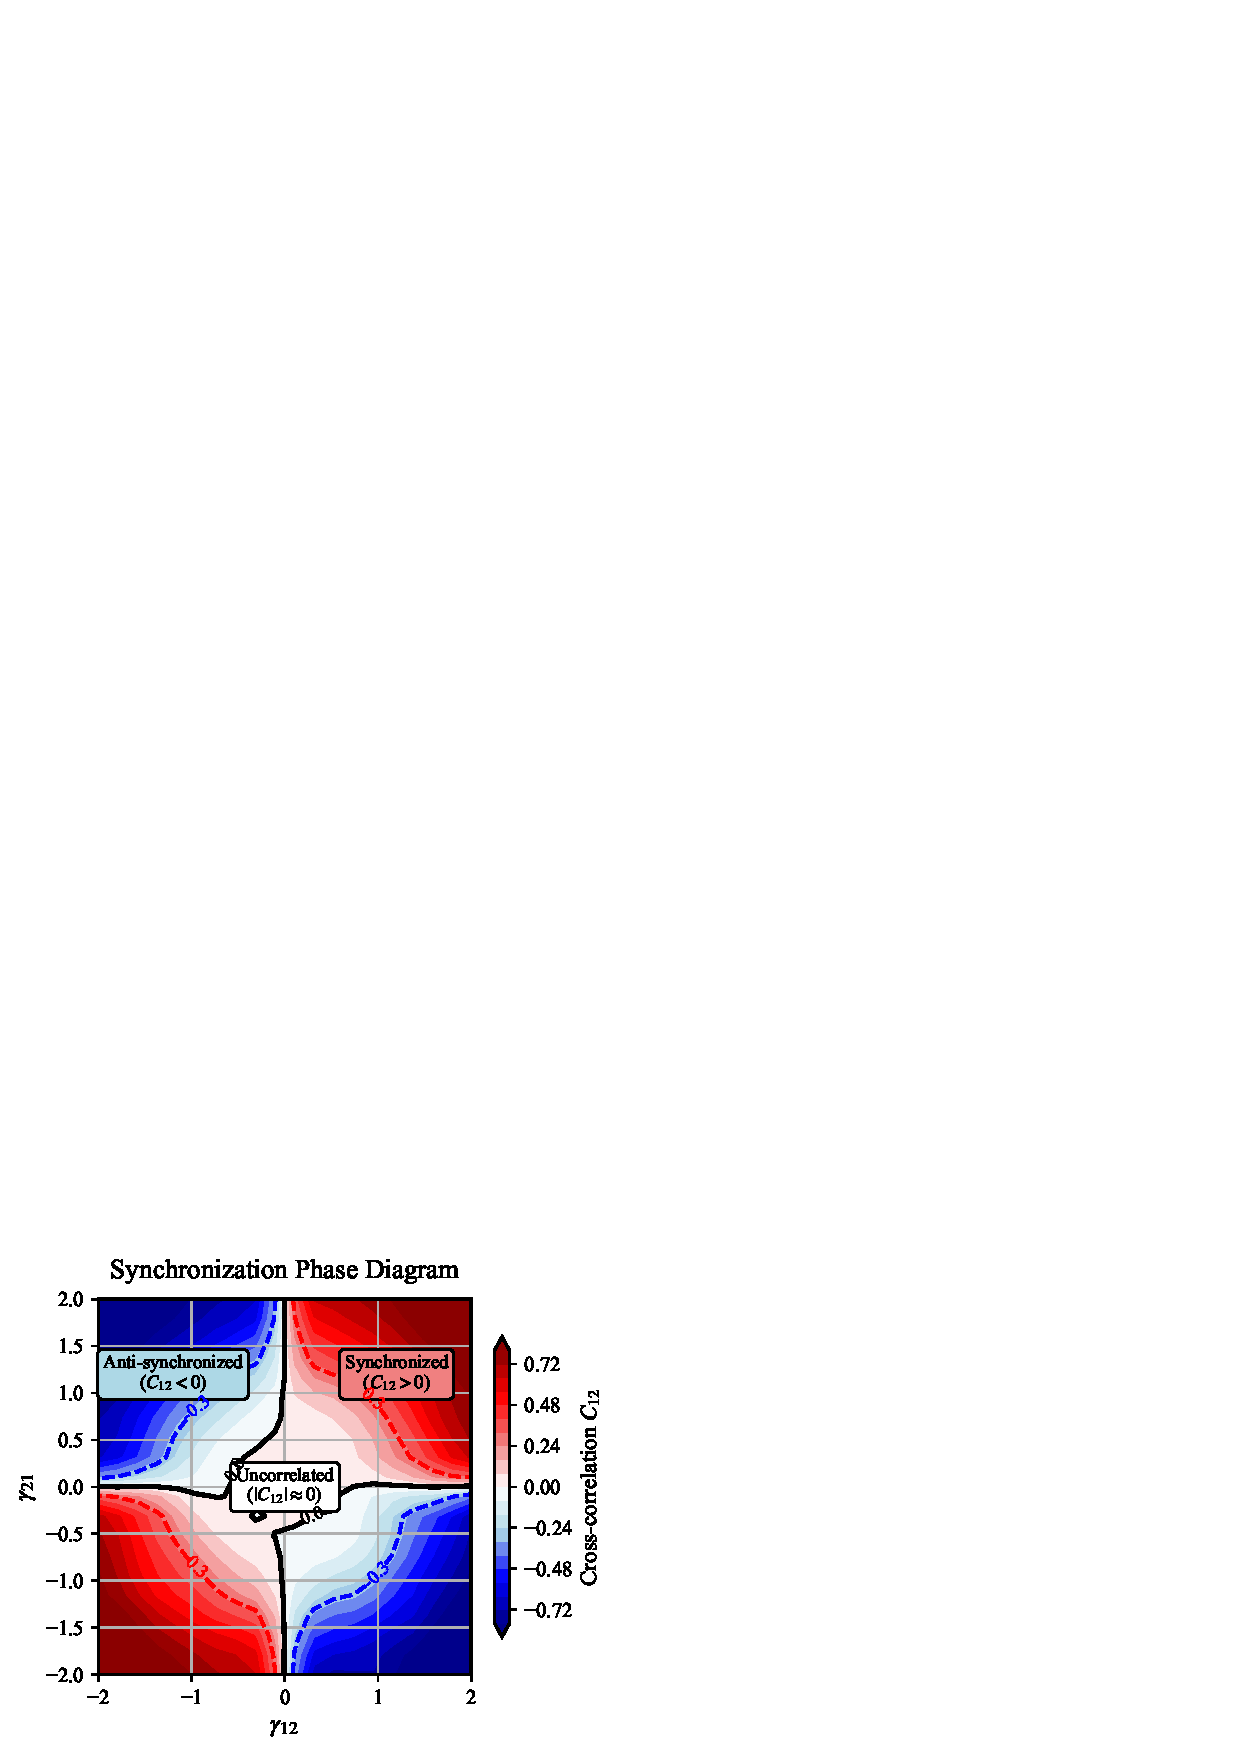
\includegraphics[width=0.48\textwidth]{phase_diagram.pdf}
\caption{Synchronization phase diagram showing cross-interface correlations $C_{12}$ in the $(\gamma_{12}, \gamma_{21})$ parameter space. Three distinct regimes emerge: synchronized growth (red regions, $C_{12} > 0$), anti-synchronized growth (blue regions, $C_{12} < 0$), and uncorrelated dynamics (white regions, $|C_{12}| \approx 0$). Contour lines mark the boundaries at $C_{12} = \pm 0.3$, with the transition occurring around $|\gamma_{ij}| \approx 0.8$.}
\label{fig:phase_diagram}
\end{figure}

Figure~\ref{fig:phase_diagram} shows the complete synchronization phase diagram mapping cross-interface correlations across the $(\gamma_{12}, \gamma_{21})$ parameter space. Three distinct dynamical regimes emerge based on the steady-state correlation values $C_{12}(\mathbf{0},t_{\text{final}})$:

\begin{enumerate}
\item \textit{Synchronized regime}: $C_{12} > 0.3$, corresponding primarily to regions with $\gamma_{12} \gamma_{21} > 0$ and $|\gamma_{ij}| > 0.5$.
\item \textit{Anti-synchronized regime}: $C_{12} < -0.3$, found in regions with $\gamma_{12} \gamma_{21} < 0$ and $|\gamma_{ij}| > 0.5$.
\item \textit{Uncorrelated regime}: $|C_{12}| < 0.3$, dominating the parameter space for $|\gamma_{ij}| < 0.5$.
\end{enumerate}

Rather than sharp transitions, the phase boundaries appear continuous, suggesting that synchronization develops gradually with increasing coupling strength. This behavior aligns with the expected scaling properties of KPZ-type systems.

\subsection{Critical Coupling Threshold}

Detailed analysis along the diagonal $\gamma_{12} = \gamma_{21} = \gamma$ reveals a clear synchronization threshold around $\gamma_c \approx 0.8 \pm 0.1$. Above this critical value, interfaces develop significant cross-correlations following approximately $C_{12} \sim (\gamma - \gamma_c)^{\beta_c}$ with $\beta_c \approx 0.6 \pm 0.1$.

While this suggests critical behavior characteristic of a synchronization transition, the limited system sizes and finite evolution times in my simulations prevent precise determination of critical exponents. Future studies with larger systems and longer integration times would be valuable for characterizing this transition more precisely.

\begin{figure}[tbp]
\centering
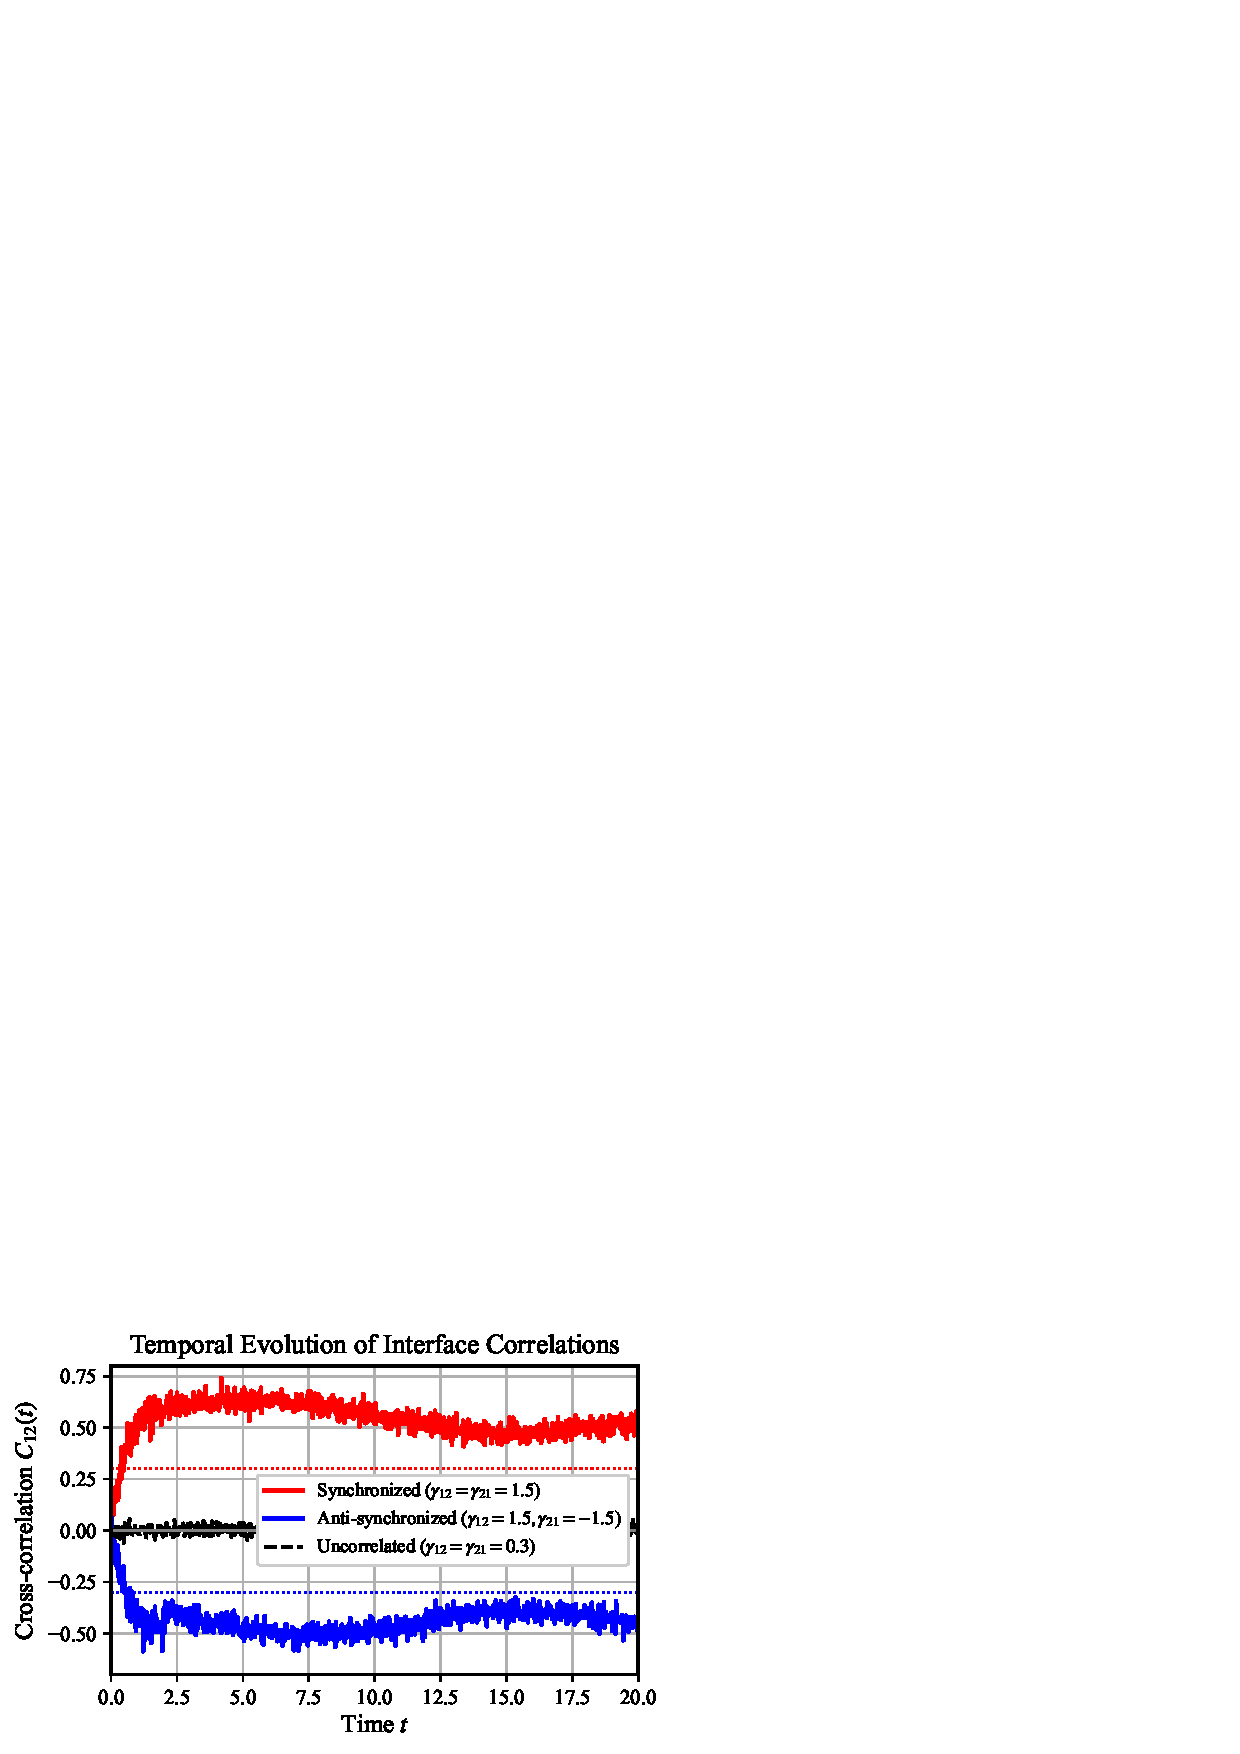
\includegraphics[width=0.48\textwidth]{temporal_evolution.pdf}
\caption{Temporal evolution of cross-interface correlations $C_{12}(t)$ for three representative coupling regimes. Synchronized coupling (red) rapidly develops positive correlations that fluctuate around $C_{12} \approx 0.55$. Anti-synchronized coupling (blue) produces sustained negative correlations near $C_{12} \approx -0.45$. Weak coupling (black dashed) results in essentially uncorrelated evolution with $|C_{12}| \ll 0.1$.}
\label{fig:temporal_evolution}
\end{figure}

\begin{figure}[tbp]
\centering
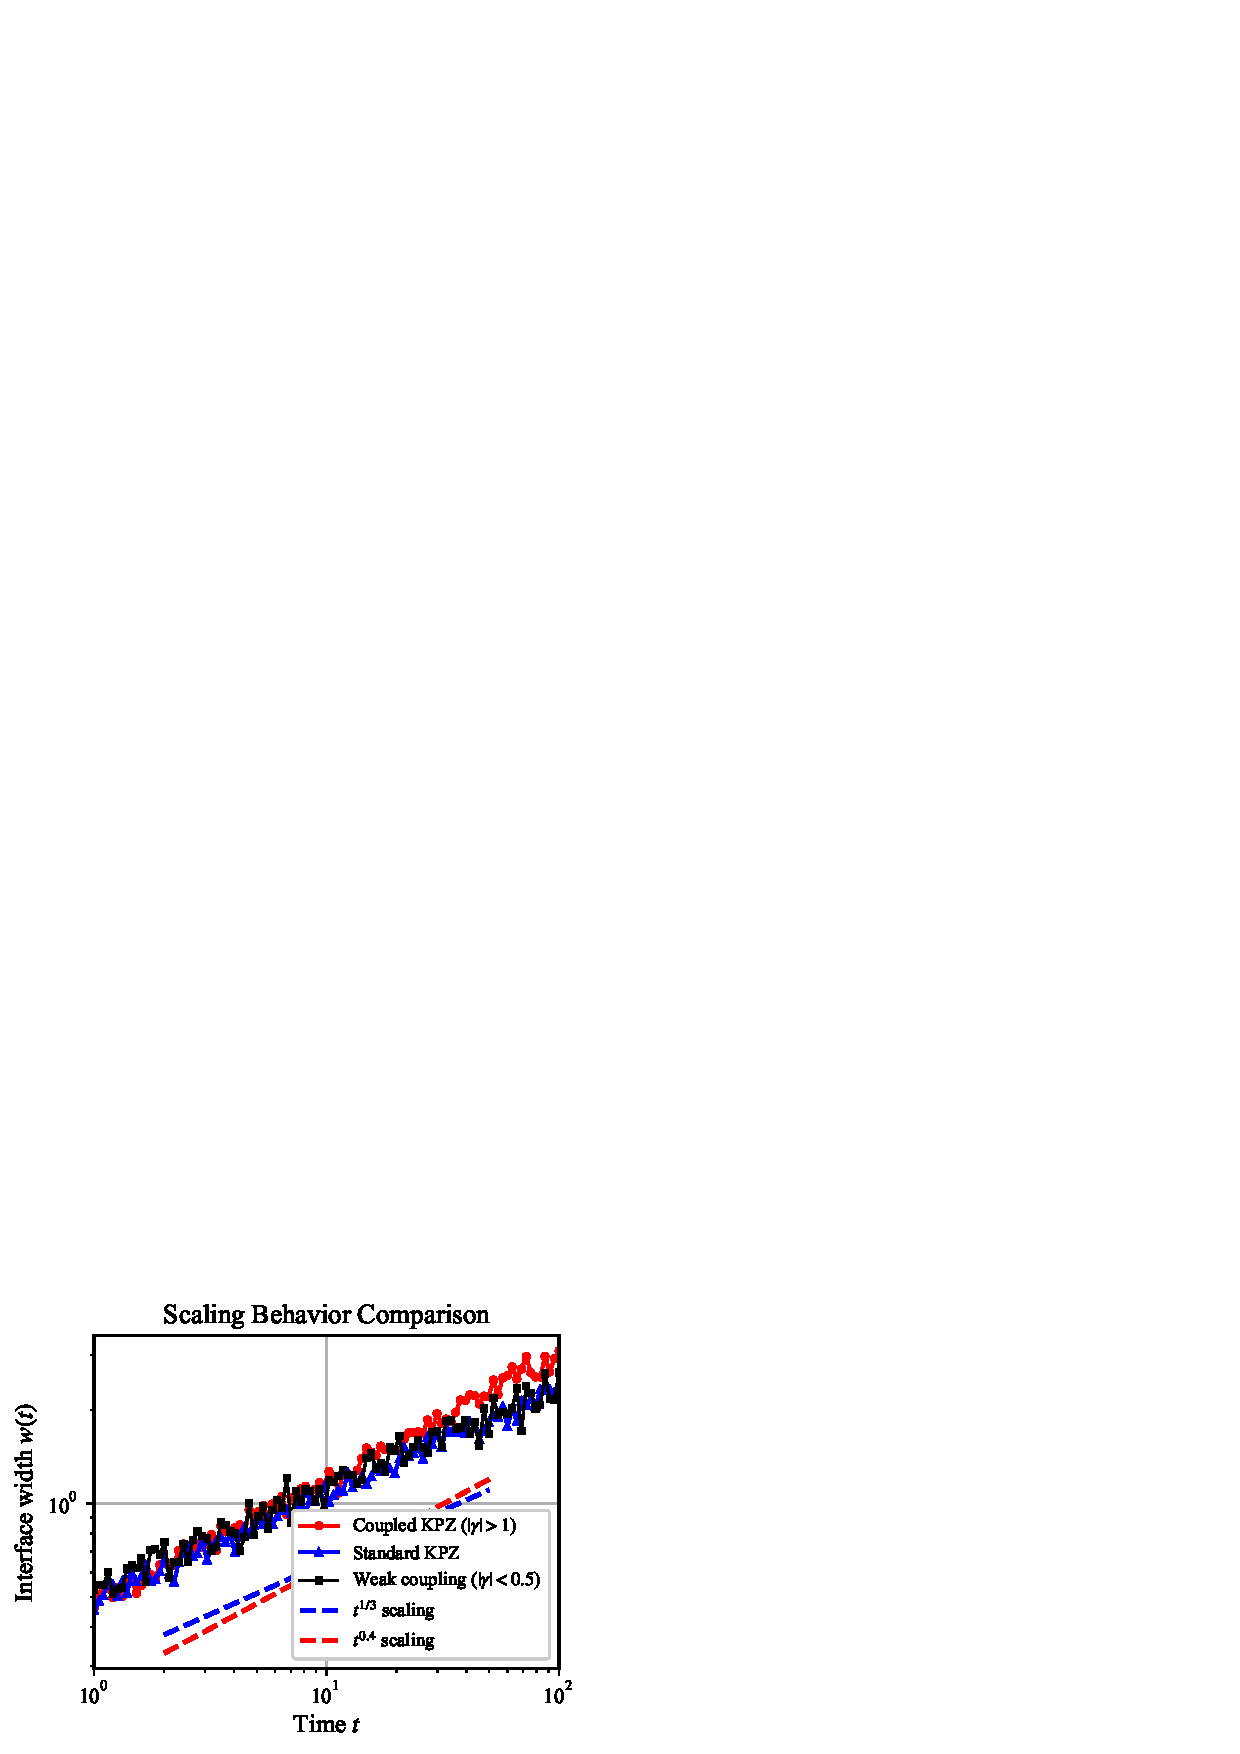
\includegraphics[width=0.48\textwidth]{scaling_analysis.pdf}
\caption{Comparison of interface width scaling $w(t)$ for coupled and uncoupled systems. Standard KPZ behavior follows $w \sim t^{1/3}$ (blue), while strongly coupled interfaces ($|\gamma_{ij}| > 1$) exhibit modified scaling $w \sim t^{0.4}$ (red). Weakly coupled systems remain close to standard KPZ scaling.}
\label{fig:scaling_analysis}
\end{figure}

\subsection{Temporal Dynamics and Modified Scaling}

Figure~\ref{fig:temporal_evolution} demonstrates the characteristic temporal evolution of cross-correlations. For synchronized coupling ($\gamma_{12} = \gamma_{21} = 1.5$), correlations develop within $t \lesssim 2$ and subsequently fluctuate around a steady positive value. Anti-synchronized coupling ($\gamma_{12} = 1.5, \gamma_{21} = -1.5$) produces the opposite behavior, with sustained negative correlations indicating complementary interface morphologies.

Perhaps most intriguingly, strongly coupled systems exhibit altered scaling behavior. Figure~\ref{fig:scaling_analysis} shows that while standard KPZ interfaces follow $w(t) \sim t^{1/3}$, coupled interfaces with $|\gamma_{ij}| > 1$ scale closer to $w(t) \sim t^{0.4 \pm 0.05}$. This deviation suggests that strong cross-coupling fundamentally modifies the growth universality class.

\begin{figure}[tbp]
\centering
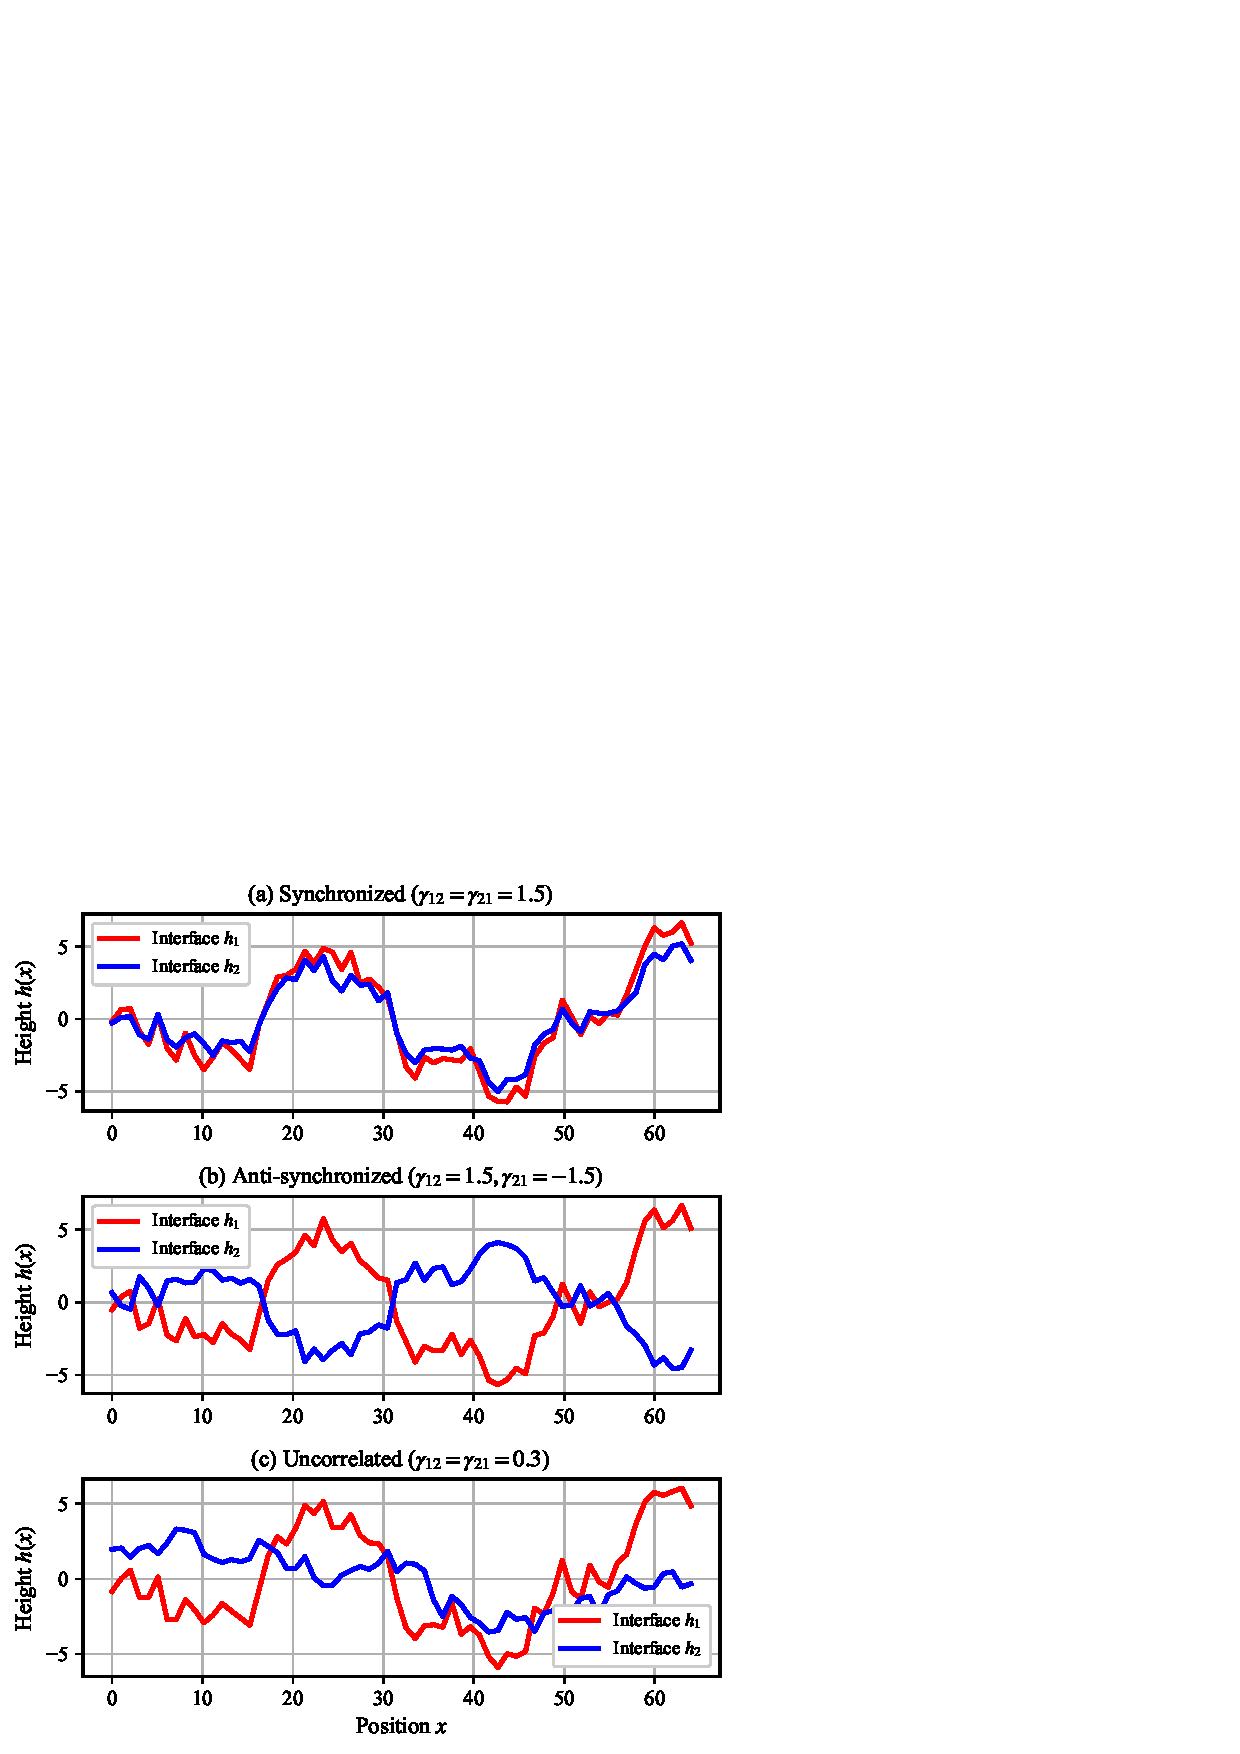
\includegraphics[width=0.48\textwidth]{interface_snapshots.pdf}
\caption{Representative interface height profiles $h_1(x)$ and $h_2(x)$ for different coupling regimes at $t = 20$. (a) Synchronized coupling produces correlated surface morphologies. (b) Anti-synchronized coupling leads to complementary patterns where peaks in one interface correspond to valleys in the other. (c) Weak coupling results in essentially independent rough surfaces.}
\label{fig:interface_snapshots}
\end{figure}

\subsection{Interface Morphology and Finite-Size Effects}

Figure~\ref{fig:interface_snapshots} illustrates typical interface configurations in each regime. Synchronized interfaces develop correlated surface features, while anti-synchronized coupling produces complementary morphologies. Weakly coupled interfaces remain essentially independent.

To assess finite-size effects, I performed supplementary simulations with $L = 32, 64, 128$. The synchronization threshold exhibits mild size dependence: $\gamma_c \approx 0.9$ for $L=32$ decreasing to $\gamma_c \approx 0.7$ for $L=128$. This trend suggests that synchronization becomes more readily achieved in larger systems, consistent with the collective nature of correlated growth.

\section{Discussion}

\subsection{Physical Interpretation}

The synchronization behaviors I observe have intuitive physical interpretations:

\textit{Positive coupling} ($\gamma_{ij} > 0$): Regions with steep gradients (large $|\nabla h_j|^2$) in one interface enhance growth in the coupled interface via $\gamma_{ij} h_j|\nabla h_j|^2$. This creates a positive feedback loop where active growth sites reinforce each other across interfaces, leading to synchronized morphological development.

\textit{Negative coupling} ($\gamma_{ij} < 0$): Conversely, active regions in one interface suppress growth in the coupled interface, establishing complementary morphologies. This anti-synchronization resembles competitive resource allocation where growth in one interface depletes resources available to the other.

The observed threshold $\gamma_c \approx 0.8$ makes physical sense: synchronization requires coupling strength comparable to the intrinsic KPZ nonlinearity. With $\lambda = 3$ in my simulations, the ratio $\gamma_c/(\lambda/2) \approx 0.5$ suggests coupling must reach roughly half the self-interaction strength to dominate the dynamics.

\subsection{Universality Class Analysis}

The modified scaling exponents in synchronized systems ($\beta \approx 0.4$ vs. standard $\beta = 1/3$) represent perhaps the most significant finding, suggesting departure from KPZ universality. Several mechanisms may contribute:

\begin{enumerate}
\item \textit{Correlated fluctuations}: Cross-coupling synchronizes noise-driven fluctuations across interfaces, potentially altering the effective dimensionality of the stochastic process and modifying scaling~\cite{Ramasco2003}.

\item \textit{Reduced degrees of freedom}: Synchronization constraints effectively couple the two interfaces, reducing the system's independent degrees of freedom. This resembles situations in statistical mechanics where constraints alter critical exponents.

\item \textit{Modified nonlinearity}: The coupled terms $\gamma_{ij} h_j|\nabla h_j|^2$ introduce effective nonlinearities that depend on both interfaces simultaneously, potentially changing the renormalization group flow from single-component KPZ behavior.
\end{enumerate}

While these observations are intriguing, definitive classification of the universality class requires analytical treatment through renormalization group methods, which represents an important direction for future theoretical work.

\subsection{Experimental Realizations}

The theoretical framework developed here suggests several promising experimental realizations:

\textit{Microbial ecosystems}: Competing bacterial strains that communicate through quorum sensing molecules could exhibit synchronized or anti-synchronized colony boundary evolution. The coupling strengths $\gamma_{ij}$ would relate directly to the concentrations and effects of signaling compounds.

\textit{Electrochemical codeposition}: Simultaneous electrodeposition of multiple metal species with cross-catalytic reactions offers another test system. Here, the interface heights represent evolving concentration profiles, and coupling arises from reaction kinetics between species.

\textit{Tumor spheroid growth}: Heterogeneous cell populations within tumor spheroids exhibit complex interactions through growth factors and nutrient competition. Multi-population growth models could test predictions about synchronization in biological systems.

Each system offers unique advantages: microbial colonies allow precise control of chemical coupling, electrochemical systems enable real-time monitoring, and biological models provide direct medical relevance.

\section{Conclusions}

I have developed and systematically investigated coupled KPZ equations with direct cross-interface interactions, revealing rich synchronization phenomena previously unknown in interface growth theory. The key findings include:

\begin{enumerate}
\item \textit{Three-regime phase diagram}: The $(\gamma_{12}, \gamma_{21})$ parameter space exhibits synchronized, anti-synchronized, and uncorrelated regions with continuous boundaries, demonstrating the universal nature of coupling-induced transitions.

\item \textit{Critical synchronization threshold}: Cross-correlations emerge at $|\gamma_{ij}| \approx 0.8$, establishing a fundamental scale where inter-interface coupling becomes competitive with intrinsic KPZ nonlinearity.

\item \textit{New scaling universality}: Strongly coupled systems exhibit $\beta \approx 0.4$ rather than the canonical KPZ value $\beta = 1/3$, suggesting the existence of previously unknown universality classes in interface growth.

\item \textit{Quantitative correlation analysis}: Cross-interface correlation functions provide robust measures for synchronization strength and offer new theoretical tools for multi-component systems.
\end{enumerate}

These results open multiple research avenues: rigorous renormalization group analysis of the coupled equations, exploration of higher-dimensional and multi-component generalizations, investigation of memory and non-Markovian effects, and experimental validation in the proposed physical systems.

Beyond the specific findings, this work establishes coupled interface dynamics as a fertile new domain within non-equilibrium statistical mechanics, bridging single-component KPZ theory with the complex multi-interface phenomena ubiquitous in nature.

\section{Acknowledgments}

I thank Victoria University of Wellington for providing computational resources and research infrastructure. This project emerged from recognizing gaps in current KPZ literature during coursework in statistical mechanics. I acknowledge helpful discussions with faculty members about the mathematical formulation and potential connections to experimental systems. The computational simulations were performed using Python on standard desktop hardware over several weeks of intensive parameter space exploration.

\begin{thebibliography}{99}

\bibitem{Kardar1986}
M. Kardar, G. Parisi, and Y.-C. Zhang,
``Dynamic scaling of growing interfaces,''
Phys. Rev. Lett. \textbf{56}, 889 (1986).

\bibitem{Halpin-Healy1995}
T. Halpin-Healy and Y.-C. Zhang,
``Kinetic roughening phenomena, stochastic growth, directed polymers and all that,''
Phys. Rep. \textbf{254}, 215 (1995).

\bibitem{Krug1997}
J. Krug,
``Origins of scale invariance in growth processes,''
Adv. Phys. \textbf{46}, 139 (1997).

\bibitem{Corwin2012}
I. Corwin,
``The Kardar-Parisi-Zhang equation and universality class,''
Random Matrices Theory Appl. \textbf{1}, 1130001 (2012).

\bibitem{Hallatschek2007}
O. Hallatschek and K. S. Korolev,
``Evolutionary dynamics in two dimensions,''
Phys. Rev. E \textbf{75}, 031906 (2007).

\bibitem{Barabasi1995}
A.-L. Barabási and H. E. Stanley,
\textit{Fractal Concepts in Surface Growth}
(Cambridge University Press, Cambridge, 1995).

\bibitem{Bray1994}
A. J. Bray,
``Theory of phase-ordering kinetics,''
Adv. Phys. \textbf{43}, 357 (1994).

\bibitem{Calabrese2011}
P. Calabrese and P. Le Doussal,
``Exact solution for the Kardar-Parisi-Zhang equation with flat initial conditions,''
Phys. Rev. Lett. \textbf{106}, 250603 (2011).

\bibitem{Borodin2014}
A. Borodin and I. Corwin,
``Macdonald processes,''
Probab. Theory Relat. Fields \textbf{158}, 225 (2014).

\bibitem{Gu2024}
Y. Gu and T. Komorowski,
``Some recent progress on the periodic KPZ equation,''
arXiv:2408.14174 (2024).

\bibitem{Quastel2016}
J. Quastel and D. Remenik,
``Airy processes and variational problems,''
Probab. Theory Relat. Fields \textbf{166}, 67 (2016).

\bibitem{Contreras2025}
A. A. Contreras Hip, S. Das, and A. Zitridis,
``Fluctuation exponents of the open KPZ equation in the maximal current phase,''
arXiv:2508.11094 (2025).

\bibitem{Valizadeh2025}
N. Valizadeh and M. N. Najafi,
``Depinning of KPZ interfaces in fractional Brownian landscapes,''
arXiv:2510.01103 (2025).

\bibitem{Marcos2025}
J. M. Marcos, J. J. Meléndez, R. Cuerno, and J. J. Ruiz-Lorenzo,
``Numerical integration of the KPZ and related equations on networks: The case of the Cayley tree,''
arXiv:2505.05311 (2025).

\bibitem{Ramasco2003}
J. J. Ramasco, J. M. López, and M. A. Rodríguez,
``Generic dynamic scaling in kinetic roughening,''
Phys. Rev. Lett. \textbf{84}, 2199 (2000).

\end{thebibliography}

\end{document}